\documentclass[a4paper,11pt]{article}
\usepackage{nopageno} % visto che in questo caso abbiamo una pagina sola
\usepackage{lmodern}
\renewcommand*\familydefault{\sfdefault}
\usepackage{sfmath}
\usepackage[utf8]{inputenc}
\usepackage[T1]{fontenc}
\usepackage[italian]{babel}
\usepackage{subcaption}
\DeclareCaptionFormat{custom}
{%
    \begin{minipage}{0.65\textwidth}\textbf{#1#2}\textit{\small #3}\end{minipage}
}
\captionsetup{format=custom}
\usepackage{indentfirst}
\usepackage{graphicx}
\usepackage{animate}
\usepackage{tikz}
\usepackage{wrapfig}
\newcommand*\circled[1]{\tikz[baseline=(char.base)]{
		\node[shape=circle,draw,inner sep=2pt] (char) {#1};}}
\usepackage{enumitem}
% \usepackage[group-separator={\,}]{siunitx}
\usepackage[left=2cm, right=2cm, bottom=2cm]{geometry}
\frenchspacing

\newcommand{\num}[1]{#1}

% Macro varie...
\newcommand{\file}[1]{\texttt{#1}}
\renewcommand{\arraystretch}{1.3}
\newcommand{\esempio}[2]{
\noindent\begin{minipage}{\textwidth}
\begin{tabular}{|p{5cm}|p{11cm}|}
	\hline
	\textbf{da \file{stdin}} & \textbf{su \file{stdout}}\\
	\hline
	\tt \small #1 &
	\tt \small #2 \\
	\hline
\end{tabular}
\end{minipage}
}

\newcommand{\sezionetesto}[1]{
    \section*{#1}
}

\newcommand{\gara}{Esame algoritmi 2022-09-20 VR}

%%%%% I seguenti campi verranno sovrascritti dall'\include{nomebreve} %%%%%
\newcommand{\nomebreve}{}
\newcommand{\titolo}{}

% Modificare a proprio piacimento:
\newcommand{\introduzione}{
%    \noindent{\Large \gara{}}
%    \vspace{0.5cm}
    \noindent{\Huge \textbf \titolo{}~(\texttt{\nomebreve{}})}
    \vspace{0.2cm}\\
}

\begin{document}

\renewcommand{\nomebreve}{convoglio}
\renewcommand{\titolo}{La battaglia del convoglio - {\large ripreso dalle OII 2012}\\}

\introduzione{}

Tra il 7 e il 10 marzo del 1943 avvenne nell'Atlantico la più grande battaglia di convogli ad oggi mai combattuta. Dei sottomarini tedeschi si comunicavano, in maniera cifrata, le posizioni delle navi di un convoglio americano da attaccare, ma questi messaggi erano decifrati dalla macchina Bomba ideata da Turing per rompere il codice di Enigma.

Abbiamo $N$ navi e gli $N$ messaggi ad esse relativi, ciascuno coi dettagli per l'attacco alla nave che gli corrisponde. Dal testo dei messaggi non è tuttavia sempre possibile risalire alla nave cui essi si riferiscono. Si assuma che una corrispondenza sia stata ricostruita, ma di voler controllare se essa sia l'unica possibile o meno.
Nell'esempio in figura (dove $N=3$), il primo messaggio può riferirsi sia alla prima ($S0$) che alla terza ($S2$) nave, così come il secondo messaggio; invece il terzo messaggio ($M2$) è compatibile con la seconda ($S1$) oppure con la terza ($S2$) nave. 
    
\begin{figure}[h!]
  \centering
  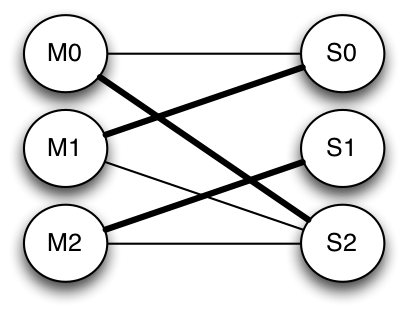
\includegraphics{figura.png}
  \caption{Rappresentazione di un'istanza: coppie compatibili (tutte le linee) e corrispondenza biunivoca (le solo linee in grassetto).}
\end{figure}

Sempre in figura, le associazioni in linea spessa (le 3 coppie messaggio-nave compatibili $M0-S2$, $M1-S0$, e $M2-S1$) evidenziano una possibile \textbf{corrispondenza biunivoca} tra i messaggi e le navi, dove \emph{ad ogni messaggio distinto corrisponde una nave distinta}. Questa e' una corrispondenza biunivoca in quanto:

\begin{itemize}
  
    \item  per ogni $i=1,2,3$ esiste uno ed un solo $j$ tale che la coppia $Mi-Sj$ e' stata inclusa;
    \item  per ogni $j=1,2,3$ esiste uno ed un solo $i$ tale che la coppia $Mi-Sj$ e' stata inclusa.
\end{itemize}


    Dobbiamo accertarci che non esistano altre corrispondenze biunivoche interamente costituite da coppie messaggio-nave compatibili per la data istanza (rappresentate in figura da archi $Mi-Sj$, sia in grassetto che in tratto semplice).
    Per esempio, nel caso della Figura 1, esiste anche una seconda corrispondenza biunivoca: $M0-S0$, $M1-S2$, $M2-S1$.
    
    Aiuta Turing a capire se la corrispondenza biunivoca assegnata (quella in grassetto) sia anche unica!

\newpage
\sezionetesto{Input ed Output}

Input ed output avvengono da \verb'stdin' e su \verb'stdout' rispettivamente.



\sezionetesto{Input}

La struttura dello stream in input è la seguente: la prima riga contiene $2$ interi separati da spazio, nell'ordine: il numero di navi $N$ (che coincide con il numero dei messaggi intercettati) e il numero complessivo $M$ di coppie messaggio-nave compatibili. I messaggi sono identificati da interi compresi tra $0$ e $N-1$, e anche le navi sono identificate da interi compresi tra $0$ e $N-1$.

Le successive $M$ righe contengono ciascuna una coppia ordinata di interi rappresentanti, rispettivamente, un messaggio e una nave compatibile ad esso. Di queste $M$ righe, le prime $N$ rappresentano la corrispondenza biunivoca trovata da Turing.  
    
\sezionetesto{Output}

Se non esiste nessuna altra corrispondenza possibile, lo stream in output deve essere costituito da una sola linea, contenente l'intero $-1$. Altrimenti, se esiste un'altra corrispondenza biunivoca ammissibile, lo stream consiste di $N$ linee che la codificano come lista di coppie di interi, messaggio e nave, separate da spazio e ordinate per numero di messaggio.



% Esempi
\sezionetesto{Esempio di input/output}

In attachment alla pagina del problema trovate diverse coppie input/output tra cui le seguenti.

Con riferimento alla figura, rappresentando i messaggi M0, M1 e M2 con gli interi 0,1 e 2, e  le navi S0, S1 e S2 con gli interi 0,1 e 2, l'istanza nella figura viene rappresentata dal seguente stream, posto a sinistra.
  Lo stream a destra codifica una seconda corrispondenza biunivoca ammissibile e costituisce pertanto una risposta valida.

\vspace{0.5cm}
\esempio{3 6

  0 2

  1 0

  2 1

  0 0

  1 2

  2 2}{0 0

  1 2

  2 1}

Togliendo una sola coppia dalla lista delle coppie messaggio-nave compatibili, ci ritroviamo in un caso dove l'unica corrispondenza biunivoca valida era quella assegnata in input.

\vspace{0.5cm}
\esempio{3 5
  
  0 2
  
  1 0
  
  2 1
  
  1 2
  
  2 2
}{-1}

\newpage
 Nel caso le risposte valida fossero più di una vi basta fornirne una qualsiasi. Nel seguente esempio sarebbe altrettanto corretto l'output che si è dato nel primo esempio sopra. 

\vspace{0.5cm}
\esempio{3 7
  
  0 2

  1 0

  2 1

  1 1

  0 0

  1 2

  2 2}{0 0

  1 1

  2 2}


\section*{Subtask}

  \begin{itemize}
  \item \textbf{Subtask 1 [0 punti]:} i casi di esempio forniti alla pagina del problema, essi includono i 2 casi sopra.
      \vspace{-0.6cm}
       \begin{center}
      \rule{0.5\textwidth}{0.4pt} \hfill  \hfill \hfill
       \end{center}
      \vspace{-0.6cm}      
    \item \textbf{Subtask 2 [15 punti]:} $M=N+2$.
    \item \textbf{Subtask 3 [20 punti]:} ciascuna nave e ciascun messaggio appare al più $2$ volte nella lista delle possibili corrispondenze (quindi, $M \leq 2N$).
    \item \textbf{Subtask 4 [25 punti]:} $N \leq  3.000$, $M \leq  5.000$.
    \item \textbf{Subtask 5 [40 punti]:} $N \leq  100.000$, $M \leq  200.000$.
  \end{itemize}


\end{document}
